\section{Methodology}
\label{sec:methodology}

Figure~\ref{fig:system_overview} summarizes the complete setup of the thesis.

\begin{figure}[H]
\centering
\resizebox{\textwidth}{!}{%
\begin{tikzpicture}[font=\footnotesize]

% ---------------- stage 1: data sources ----------------
\node[fgdata=2.7cm, minimum height=1.95cm] (wx)  at (0, 3.1)
  {\textbf{Weather forecasts}\\ICON-D2 from\\DWD, Open-Meteo};
\node[fgdata=2.7cm, minimum height=1.95cm] (ent) at (0, 1.03)
  {\textbf{\mbox{ENTSO-E} data}\\prices, load, generation,\\load forecast};
\node[fgdata=2.7cm, minimum height=1.95cm] (mkt) at (0,-1.03)
  {\textbf{Market data}\\reserve auctions,\\EXAA prices};
\node[fgdata=2.7cm, minimum height=1.95cm] (geo) at (0,-3.1)
  {\textbf{Geodata}\\MaStR capacity,\\Eurostat population};

% ---------------- stage 2: input assembly ----------------
\node[fgproc=1.9cm, minimum height=7.9cm] (asm) at (3.2, 0)
  {\textbf{Assembly of the admissible information set}\\[6pt]
   only inputs observable at the forecast creation time \(t \le\) 12:00};

% ---------------- stage 3: component models ----------------
\node[fgproc=2.75cm] (mload) at (6.2, 2.35)
  {\textbf{OBTF}\\\textbf{load model}\\direct, or correction of the \mbox{ENTSO-E} forecast};
\node[fgproc=2.75cm] (msol)  at (6.2, 0)
  {\textbf{OBTF}\\\textbf{solar model}\\capacity-weighted\\weather};
\node[fgproc=2.75cm] (mwind) at (6.2,-2.35)
  {\textbf{OBTF}\\\textbf{wind model}\\hub-height wind fields};

% ---------------- stage 4: component forecasts ----------------
\node[fgout=1.25cm] (fl) at (8.9, 2.35) {\(\hat{L}_{d,q|d-1}\)\\load};
\node[fgout=1.25cm] (fs) at (8.9, 0)    {\(\hat{S}_{d,q|d-1}\)\\solar};
\node[fgout=1.25cm] (fw) at (8.9,-2.35) {\(\hat{W}_{d,q|d-1}\)\\wind};
\begin{scope}[on background layer]
  \node[fggroup, fit=(fl)(fs)(fw)] (grp) {};
\end{scope}
% ---------------- stage 5: price model and forecast ----------------
\node[fgproc=2.2cm] (mprice) at (11.8, 0)
  {\textbf{Price model}};
\node[fgout=1.6cm] (fp) at (11.8,-2.35)
  {\(\hat{P}_{d,q|d-1}\)\\price forecast};

% ---------------- stage 6: evaluation and deployment ----------------
\node[fgdata=2.7cm, minimum height=1.45cm] (post) at (0,-5.1)
  {\textbf{Realized values}};
\node[fgdata=2.7cm, minimum height=1.45cm] (postent) at (0,-6.8)
  {\textbf{\mbox{ENTSO-E} solar and\\wind forecasts}};
\node[fgeval=3.7cm] (eval) at (4.4,-5.95)
  {\textbf{Thesis evaluation}\\1~Feb to 31~Jul~2026\\RMSE, MAE, Giacomini--White tests\\for RQ1, RQ2, and RQ3};
\node[fgext=4.3cm] (arena) at (10.4,-5.95)
  {\textbf{Energy-Arena}\\daily submission before 12:00,\\scored against realized outcomes\\on a public leaderboard};

% ---------------- flows ----------------
\foreach \s in {wx, ent, mkt, geo}
  \draw[fgflow] (\s.east) -- (\s.east -| asm.west);
\draw[fgflow] (asm.east |- mload) -- (mload.west);
\draw[fgflow] (asm.east |- msol)  -- (msol.west);
\draw[fgflow] (asm.east |- mwind) -- (mwind.west);
\draw[fgflow] (mload.east) -- (fl.west);
\draw[fgflow] (msol.east)  -- (fs.west);
\draw[fgflow] (mwind.east) -- (fw.west);
\draw[fgflow] (fl.east) -- ([yshift=4pt]mprice.west);
\draw[fgflow] (fs.east) -- (mprice.west);
\draw[fgflow] (fw.east) -- ([yshift=-4pt]mprice.west);
\draw[fgflow] (mprice.south) -- (fp.north);

% direct price-model inputs (top channel)
\draw[fgflow] (asm.north) -- ++(0,0.5) -| (mprice.north);

% forecasts to evaluation and benchmark (bus)
\coordinate (bus) at (0,-4.4);
\draw[thick, draw=fgLine] (grp.south) -- (grp.south |- bus);
\draw[thick, draw=fgLine] (fp.south)  -- (fp.south |- bus);
\draw[thick, draw=fgLine] (5.4,0 |- bus) -- (fp.south |- bus);
\draw[fgflow] (5.4,0 |- bus) -- (5.4,0 |- eval.north);
\draw[fgflow] (arena.north |- bus) -- (arena.north);
\draw[fgflow] (post.east) -- (post.east -| eval.west);
\draw[fgflow] (postent.east) -- (postent.east -| eval.west);

% ---------------- legend (two rows) ----------------
\begin{scope}[shift={(0.2,-8.5)}]
  \node[fgdata=0.3cm, minimum height=0.42cm] (k1) at (0,0) {};
  \node[right=3pt of k1, font=\scriptsize] {data source};
  \node[fgproc=0.35cm, minimum height=0.32cm] (k2) at (4.3,0) {};
  \node[right=3pt of k2, font=\scriptsize] {process or model};
  \node[fgout=0.3cm, minimum height=0.32cm] (k3) at (8.9,0) {};
  \node[right=3pt of k3, font=\scriptsize] {forecast (data product)};
  \node[fgeval=0.25cm, minimum height=0.32cm] (k4) at (0,-0.62) {};
  \node[right=3pt of k4, font=\scriptsize] {evaluation};
  \node[fgext=0.3cm, minimum height=0.32cm] (k5) at (4.3,-0.62) {};
  \node[right=3pt of k5, font=\scriptsize] {external platform};
  \node[fgrq=0.35cm, minimum height=0.32cm, rounded corners=2pt] (k6) at (8.9,-0.62) {};
  \node[right=3pt of k6, font=\scriptsize] {RQ};
  \node[fgout=0.3cm, minimum height=0.32cm, fgvar] (k7) at (0,-1.24) {};
  \draw[fgaux] ([xshift=3pt]k7.east) -- ++(0.55,0) coordinate (k7a);
  \node[right=2pt of k7a, font=\scriptsize] {dashed: variant or benchmark};
  \draw[fgflow] (8.65,-1.24) -- ++(0.55,0) coordinate (k8a);
  \node[right=2pt of k8a, font=\scriptsize] {data flow};
\end{scope}

\end{tikzpicture}%
}
\caption[Overview of the complete setup of the thesis.]
{Overview of the complete setup of the thesis, from the open data sources
through the forecasting models to the evaluation and the daily submission. The
legend applies to all process diagrams in this thesis.}
\label{fig:system_overview}
\end{figure}


In this setup, open data sources are assembled into the admissible information
set at the forecast creation time \(t\). This set feeds the OBTF load, solar, and wind models,
and the price model receives their forecasts together with further inputs from
the same set. All models are gradient-boosted trees. In RQ3, the pipeline is
rerun for each forecast creation time. The OBTF and price forecasts are
evaluated on the test period for RQ1 to RQ3. Data published only after gate
closure, namely the realized values and the \mbox{ENTSO-E} solar and wind
forecasts, are used only for evaluation and never as model inputs.

The pipeline is deployed operationally on the Energy-Arena platform
\cite{kleinebrahm2026energyarena}, which hosts separate forecasting challenges
for load, solar, wind, and the \mbox{DE-LU} day-ahead price, as
well as challenges tied to different forecast creation times. The pipeline
submits forecasts to each challenge every day before the corresponding
submission cutoff, which is the 12:00 gate closure for the day-ahead price
and correspondingly earlier for the challenges tied to earlier forecast
creation times. This deployment provides a live check that every model respects
the operational information cutoff and that the setup can be run end to end
under realistic timing constraints. The final configuration of each model in the
pipeline is summarized in Appendix~\ref{app:model_configs}.


\subsection{Problem Formulation}
\label{sec:problem_formulation}

This thesis considers the operational point forecasting problem of predicting
quarter-hourly day-ahead electricity prices in the \mbox{DE-LU} bidding zone. Let
\(P_{d,q}\) denote the realized day-ahead price for delivery
day \(d\) and market time unit (MTU) \(q\). On regular days, the day consists of
96 quarter-hourly MTUs, and the forecast for delivery day \(d\)
is created on day \(d-1\), the day before delivery. It must be available
before the day-ahead gate closure at
12:00 \cite{epexSpotPowerMarket}. For a forecast creation time
\(t\) on day \(d-1\), the price forecasting task is written as
\[
  \hat{P}_{d,q|d-1} = f(\mathcal{F}_{d-1}^{t}, q),
  \quad q \in \mathcal{Q}_d,
\]
where \(\hat{P}_{d,q|d-1}\) is the point forecast for delivery day \(d\),
\(\mathcal{Q}_d\) is the set of MTUs, and
\(\mathcal{F}_{d-1}^{t}\) is the information set available at time \(t\). Unless
stated otherwise, the information cutoff is set to the latest feasible
pre-gate-closure time, \(t=12{:}00\), and the forecast is computed and submitted
slightly before the 12:00 deadline.

The central idea is to generate forecasts of load, solar, and wind generation inside the same operational information set and then use them as
explicit inputs to the price model. The full notation is collected in the
List of Symbols. The OBTF forecasts are
\[
\begin{aligned}
  \hat{L}_{d,q|d-1} &= g^{\mathrm{load}}(\mathcal{F}_{d-1}^{t}, q), \\
  \hat{S}_{d,q|d-1} &= g^{\mathrm{solar}}(\mathcal{F}_{d-1}^{t}, q), \\
  \hat{W}_{d,q|d-1} &= g^{\mathrm{wind}}(\mathcal{F}_{d-1}^{t}, q).
\end{aligned}
\]
The OBTF solar and wind forecasts are combined into the OBTF renewable-generation
forecast
\[
  \hat{G}^{\mathrm{ren}}_{d,q|d-1}
  =
  \hat{S}_{d,q|d-1} + \hat{W}_{d,q|d-1},
\]
because the price responds to the total renewable feed-in that lowers residual
load rather than to the split between the two sources
(Section~\ref{sec:price_model}). Both are still forecast separately by their own
models.
Together with the OBTF load forecast, this defines the OBTF residual-load
forecast,
\[
  \widehat{RL}_{d,q|d-1}
  =
  \hat{L}_{d,q|d-1} - \hat{G}^{\mathrm{ren}}_{d,q|d-1}.
\]
The base price forecast, without the OBTF load, renewable-generation, and
residual-load forecasts, is denoted
\(\hat{P}^{\mathrm{base}}_{d,q|d-1}\). The price forecast with OBTF load and renewable-generation inputs, namely \(\hat{L}_{d,q|d-1}\),
\(\hat{G}^{\mathrm{ren}}_{d,q|d-1}\), and
\(\widehat{RL}_{d,q|d-1}\), is denoted
\(\hat{P}^{\mathrm{gen}}_{d,q|d-1}\). These objects define the comparisons
examined in the experimental design
(Section~\ref{sec:experimental_design}).

\subsection{Data}
\label{sec:data}

\subsubsection{Target Variable and Temporal Scope}
\label{sec:target_temporal_scope}

The target variable is the realized \mbox{DE-LU} day-ahead auction price \(P_{d,q}\),
measured in EUR/MWh. The German day-ahead market changed from hourly to
quarter-hourly market clearing on 1~October~2025
\cite{epexSpot15MinuteMarketCoupling}. Post-transition observations therefore
contain genuine 15-minute price variation, whereas pre-transition prices only
reflect hourly market clearing and are treated as historical proxy information
if they are used to extend a rolling training window. In that case, each hourly
price is expressed at quarter-hourly resolution by applying it to the four
quarter-hours of that hour, since pre-transition clearing set a single price for
the whole hour.

For model development and evaluation, the post-transition sample is split into
a development period and a held-out out-of-sample test period. The split, the
rolling estimation scheme, and their justification are defined in
Section~\ref{sec:experimental_design}.

All timestamped data are represented in the local market timezone
Europe/Berlin. To keep the model target dimension constant across delivery
days, daylight-saving transition days are mapped to the fixed 96-column
MTU representation used by the models: repeated autumn intervals
are averaged into their MTU, while missing spring intervals are
filled by within-day linear interpolation. The models and the reported evaluation use this fixed 96-unit representation, so
predicted and realized prices are always compared on the same grid. An
operational submission to Energy-Arena, which scores each delivery
day on its actual MTU grid of 92, 96, or 100 units on 23-, 24-, and
25-hour days, maps the 96-unit forecast back to those units on the two transition
days, dropping the interpolated spring units and expanding the averaged autumn
units to their two occurrences.

Figure~\ref{fig:target_price_characteristics} summarizes the empirical
behavior of the post-transition target series in the available descriptive
sample from 1~October~2025 to 31~July~2026. Prices are volatile and
asymmetric, with realized values ranging from -499.99 to 747.10~EUR/MWh and
5.8\% of observed MTUs taking negative values. The average
intraday profile shows lower prices around midday and higher prices during
morning and evening demand periods, which motivates the use of price lags,
calendar variables, weather information, load, and renewable generation.

\begin{figure}[htbp]
  \centering
  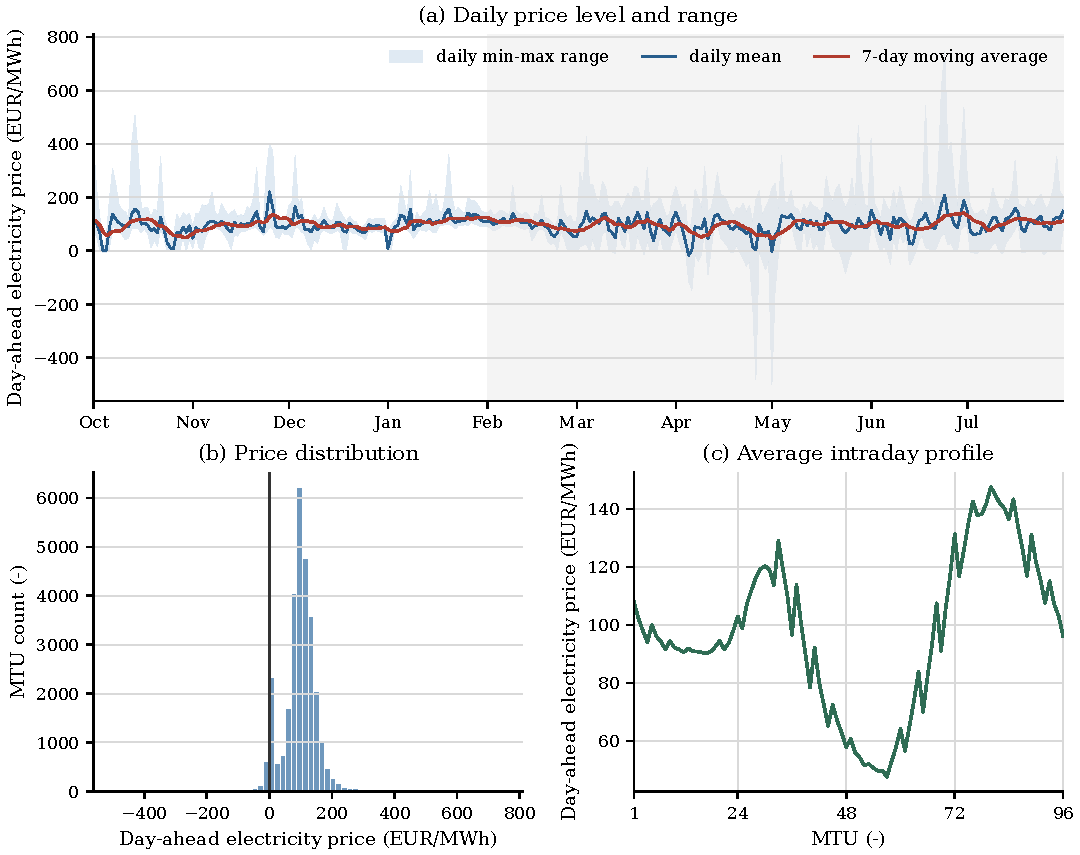
\includegraphics[width=\textwidth]{figures/target_price_characteristics.pdf}
  \caption[Empirical characteristics of the \mbox{DE-LU} day-ahead price target.]
  {Empirical characteristics of the \mbox{DE-LU} day-ahead price target in the
  available post-transition sample from 1~October~2025 to 31~July~2026. The top
  panel shows daily mean prices together with the daily minimum-maximum range
  and a seven-day moving average. The shaded area marks the fixed
  out-of-sample test period from 1~February~2026 to 31~July~2026. The lower
  panels show the empirical price distribution and the average intraday price
  profile across MTUs.}
  \label{fig:target_price_characteristics}
\end{figure}

\subsubsection{Input Data Sources and Derived Covariates}
\label{sec:input_data_sources}

The market-price data consist of realized \mbox{DE-LU} Single Day-Ahead Coupling (SDAC)
auction prices from the \mbox{ENTSO-E} Transparency Platform
\cite{entsoeTransparency}. They define the price target and provide lagged
price features that capture short-term dependence and recurring price patterns
in electricity price forecasting \cite{weron2014electricity,lago2021forecasting}.
Prices from the Energy Exchange Austria (EXAA) are treated as an
optional late market signal, because prices from this earlier auction carry
predictive information for other European day-ahead markets
\cite{ziel2015exaa}. The EXAA auction closes at 10:15
\cite{exaaTradingRules2025}, and the resulting \mbox{DE-LU} day-ahead prices are
published on the \mbox{ENTSO-E} Transparency Platform around 11:15
\cite{entsoeTransparency,eiser2026operational}.
Neighboring SDAC prices are excluded because they are released only after the
12:00 gate closure \cite{epexSpotPowerMarket}.

For the cutoff experiment, the price model also uses German control-reserve
auction results from Regelleistung.net at every cutoff after their publication
\cite{regelleistungNet2026}. Control reserve is the
balancing capacity that transmission system operators (TSOs) procure ahead of delivery
to keep grid frequency stable, split by activation speed into frequency
containment reserve (FCR), automatic frequency restoration reserve (aFRR), and manual
frequency restoration reserve (mFRR), and cleared in daily capacity auctions on the day
before delivery. The covariates summarize the published outcomes of these
auctions. They are included because capacity committed to control reserve is
withheld from the energy market and reserve prices reflect the expected scarcity
of flexible capacity. The auction outcomes are therefore expected to carry an
early signal of system tightness, which in a fundamental view shapes the
day-ahead price through the conventional supply stack \cite{pape2016fundamentals}. Together with the EXAA price signal,
these reserve-market covariates are early market signals rather than explicit
load or renewable-generation representations, so they are held out of \hyperlink{rq:component_forecast_quality}{RQ1}
and \hyperlink{rq:price_impact_generated_forecasts}{RQ2}, which study the
OBTF load and renewable-generation forecasts and their price impact without early market
information. They enter only in
\hyperlink{rq:cutoff_sensitivity}{RQ3}, where their staggered availability
across the morning is part of the information-accrual design.

Load and renewable-generation data are also obtained from \mbox{ENTSO-E}
\cite{entsoeTransparency}. For load, the pipeline uses lagged actual load,
morning actual load observed before the forecast creation time, and the public
day-ahead load forecast once it has been published before gate closure. For
renewables, realized solar generation and realized onshore and offshore wind
generation define the targets for the solar and wind forecasting models. The
\mbox{ENTSO-E} day-ahead solar and wind generation forecasts serve as
benchmarks for \hyperlink{rq:component_forecast_quality}{RQ1} but not
as price model inputs, because they are not publicly observable before gate
closure. The
publication times of all inputs and their regulatory basis are documented in
Section~\ref{sec:operational_information_set}. Load, solar, and wind are
economically relevant because demand and renewable feed-in shift the
short-run supply-demand balance and thus the merit order
\cite{sensfuss2008meritOrder}.

Weather forecasts provide the main exogenous inputs for the OBTF forecasts of
load, solar, and wind generation. The primary weather model is
\mbox{ICON-D2}, the high-resolution short-range configuration of ICON that the DWD
runs for Germany and its neighboring regions. Its forecasts are obtained both from
DWD Open Data and through the Open-Meteo API
\cite{zaengl2015icon,dwdIconForecastData,openMeteoForecastApi}. A new run starts
every three hours. Each run is named after its start time in Coordinated Universal Time (UTC), so the 06~UTC run
starts at 08:00 local summer time. A run is complete about 80~minutes after its
start, which makes the 06~UTC run available at about 09:20 local time in summer
and one hour earlier in winter. All models rely on this single weather model. The OBTF wind model additionally uses its hub-height wind
fields from Open-Meteo, described in Section~\ref{sec:wind_model}. The weather variables include
temperature, humidity, wind conditions, solar radiation, cloud cover,
precipitation, snow, and atmospheric pressure. These variables are physically
linked to load through heating and cooling demand
\cite{hong2016probabilisticLoad}, to photovoltaic generation through radiation
and cloud cover \cite{antonanzas2016pvForecasting}, and to wind generation
through wind speed and wind direction
\cite{foley2012windForecasting}. Installed renewable capacity from the
MaStR connects the weather fields to the generation fleet
\cite{bundesnetzagenturMastr}, and gridded population data from Eurostat
connect the weather fields to the demand side for load-oriented aggregation
\cite{eurostatGisco2021}. Calendar covariates comprise weekday indicators and a
German public-holiday flag taken from public-holiday calendars
\cite{pythonHolidays}.

\subsection{Operational Information Set}
\label{sec:operational_information_set}

All model inputs are restricted to information that would have been available
at the forecast creation time. For a local forecast creation time \(t\) on day
\(d-1\), the admissible information set is
\[
  \mathcal{F}_{d-1}^{t}
  =
  \left\{
    Z_{s} \mid \operatorname{avail}(Z_{s})
    \leq \tau_{d-1}^{t}
  \right\},
\]
where \(Z_{s}\) is an observation, forecast, or derived feature with reference
time \(s\), \(\operatorname{avail}(Z_{s})\) is the time at which it becomes
available to the pipeline, and \(\tau_{d-1}^{t}\) is the clock time \(t\) on day
\(d-1\). This rule is a
leakage constraint. It does not imply that every model uses every available
input.

In \hyperlink{rq:component_forecast_quality}{RQ1} and
\hyperlink{rq:price_impact_generated_forecasts}{RQ2}, forecasts are created with the
latest feasible pre-gate-closure information set
\(\mathcal{F}_{d-1}^{12:00}\), with computation and submission completed
slightly before 12:00. \hyperlink{rq:cutoff_sensitivity}{RQ3}
varies the forecast creation time over the following times on day
\(d-1\):
\[
  \mathcal{T}^{\mathrm{cut}}
  =
  \{07{:}00,08{:}00,09{:}00,10{:}00,11{:}00,12{:}00\}.
\]
At each cutoff, every input block enters only once it is published, and the
derived forecasts are rebuilt from the cutoff-specific information set.
Figure~\ref{fig:operational_timeline} summarizes the timing of the main data
blocks, Table~\ref{tab:cutoff_accrual} lists the inputs available at each
cutoff, and Appendix~\ref{app:data_timing} documents the sources behind the
availability assumptions.

The availability constraint abstracts from computation time, treating \(t\) as a
pure information cutoff and assuming the forecast is produced before gate
closure. In a strict operational sense the admissible cutoff is earlier than
\(t\) by the pipeline runtime, so a later cutoff, or a more expensive model,
trades computation time for information. In the live deployment, the creation
times \(t\) are the submission deadlines of the corresponding Energy-Arena
challenges \cite{kleinebrahm2026energyarena}. Each model run starts 20~minutes
before its deadline and submits before it, so the operational information cutoff
lies up to 20~minutes before \(t\). Because the pipeline relies on lightweight
boosted-tree models, this budget is short relative to the one-hour spacing of the
cutoff grid, and the cutoff experiment isolates the value of information rather
than a computation-time budget.

\begin{figure}[htbp]
\centering
\resizebox{0.97\textwidth}{!}{%
\begin{tikzpicture}[
    >=Latex,
    font=\small,
    rowlabel/.style={anchor=east, align=right, font=\small},
    event/.style={circle, fill=black, inner sep=1.6pt},
    gen/.style={circle, draw=black, fill=white, inner sep=1.6pt},
    note/.style={font=\footnotesize, inner sep=1.5pt, fill=white},
    stream/.style={very thick},
    cutoff/.style={dashed, gray}
]

% time-to-x mapping: x = t - 6, local clock time t on day d-1

% ---- cutoff grid and gate closure ----
\foreach \t in {7, 8, 9, 10, 11} {
  \draw[cutoff] ({\t-6},0.3) -- ({\t-6},9.7);
}
\draw[very thick] (6.0,0.3) -- (6.0,9.7);
\node[note, anchor=south west] at (6.12,9.6) {Day-ahead gate closure, 12:00};

% ---- time axis ----
\draw[->, thick] (-0.2,0) -- (6.85,0);
\foreach \t/\l in {6/06:00, 7/07:00, 8/08:00, 9/09:00, 10/10:00, 11/11:00,
                   12/12:00} {
  \draw ({\t-6},0.08) -- ({\t-6},-0.08)
    node[below, font=\footnotesize] {\l};
}
\node[font=\footnotesize] at (3.6,-1.05)
  {local time on the day before delivery};

% ---- data rows ----
\node[rowlabel] at (-0.45,0.9) {DWD ICON-D2\\weather runs};
\node[event] at (0.35,0.9) {};
\node[note, anchor=south] at (0.35,1.04) {03 UTC};
\node[event] at (3.35,0.9) {};
\node[note, anchor=south] at (3.35,1.04) {06 UTC};
\node[event] at (6.35,0.9) {};
\node[note, anchor=south] at (6.35,1.04) {09 UTC};

\node[rowlabel] at (-0.45,1.95) {ENTSO-E realized load};
\draw[stream,->] (0,1.95) -- (6.0,1.95);
\node[note, anchor=south west] at (0.05,2.05)
  {extends with up to 1 h publication delay};

\node[rowlabel] at (-0.45,3.0) {ENTSO-E realized wind\\and solar generation};
\draw[stream,->] (0,3.0) -- (6.0,3.0);
\node[note, anchor=south west] at (0.05,3.1)
  {extends with up to 1 h publication delay};

\node[rowlabel] at (-0.45,4.05) {ENTSO-E day-ahead\\load forecast};
\node[event] at (4.5,4.05) {};
\node[note, anchor=west] at (4.62,4.05) {available around 10:30};

\node[rowlabel] at (-0.45,5.1) {Control-reserve\\auction results};
\node[event] at (3.0,5.1) {};
\node[note, anchor=south] at (3.0,5.24) {FCR};
\node[event] at (4.0,5.1) {};
\node[note, anchor=south] at (4.0,5.24) {aFRR};
\node[event] at (5.0,5.1) {};
\node[note, anchor=south] at (5.0,5.24) {mFRR};

\node[rowlabel] at (-0.45,6.15) {EXAA day-ahead prices};
\node[event] at (5.25,6.15) {};
\node[note, anchor=east] at (5.13,6.15) {published around 11:15};

\node[rowlabel] at (-0.45,7.2) {Day-ahead\\auction results};
\node[event] at (6.35,7.2) {};
\node[note, anchor=east] at (6.23,7.2) {released after 12:00};

\node[rowlabel] at (-0.45,8.25) {ENTSO-E day-ahead wind\\and solar forecast};
\node[event] at (6.35,8.25) {};
\node[note, anchor=east, align=right] at (6.23,8.25)
  {publicly available after\\12:00, by 18:00};

% ---- model-run row ----
\node[rowlabel] at (-0.45,9.3) {Forecast\\creation};
\foreach \t in {7, 8, 9, 10, 11, 12} {
  \node[gen] at ({\t-6},9.3) {};
}

% ---- legend ----
\node[event] at (-1.05,-1.85) {};
\node[note, anchor=west] at (-0.9,-1.85) {publication event or deadline};
\draw[stream,->] (3.2,-1.85) -- (3.6,-1.85);
\node[note, anchor=west] at (3.75,-1.85) {extending data stream};
\node[gen] at (-1.05,-2.55) {};
\node[note, anchor=west, align=left] at (-0.9,-2.55)
  {forecast creation time};

\end{tikzpicture}%
}
\caption[Operational overview of data availability and forecast creation
times on the day before delivery.]
{Operational overview of data availability, forecast creation times, and
model runs on the day before delivery
\cite{euRegulation543_2013,kleinebrahm2026energyarena,exaaTradingRules2025,dwdIconForecastData,openMeteoForecastApi}.
The dashed grid marks the forecast creation times in local time.
Times are shown for summer time. Events to the right of 12:00 are not drawn to
scale.}
\label{fig:operational_timeline}
\end{figure}


\subsection{Forecasting Models}
\label{sec:component_forecast_models}

All learned forecasting tasks in this thesis use gradient-boosted regression
trees \cite{friedman2001gbm}. The same model family is used for load, solar,
wind, and price forecasting, which keeps the methodology consistent across
tasks. Gradient-boosted trees are well suited to the heterogeneous tabular
feature sets used here, on which they remain a strong and frequently superior
alternative to deep-learning models
\cite{grinsztajn2022tree,shwartzziv2022tabular}.
Boosted trees handle nonlinear relationships and interactions between
weather, calendar, lagged values, and market variables without requiring these
interactions to be specified manually
\cite{hastie2009elements,friedman2001gbm}. The implementation uses
efficient histogram-based boosted-tree regressors from scikit-learn and
LightGBM \cite{pedregosa2011sklearn,ke2017lightgbm}. Because both estimators
belong to the same model family, the estimator choice is treated as an
implementation detail and not as a separate research comparison.

\subsubsection{Weather Representations}
\label{sec:weather_representations}

All models use the DWD \mbox{ICON-D2} forecast as their weather input
(Section~\ref{sec:data}). \mbox{ICON-D2} is a gridded numerical weather
prediction that reports several weather variables at many grid points across
the bidding zone, mostly
at hourly resolution and for solar radiation at quarter-hourly resolution. Used
directly, the
number of raw grid features would far exceed the at most a few hundred daily
training observations in the rolling training window, a regime in which boosted
trees tend to overfit noise rather than learn the weather-to-target relationship. Because neighboring grid
points are strongly correlated, most of this dimensionality is redundant. Each
field is therefore converted into a fixed set of model features before it enters
the load, solar, wind, and price models: the grid points are grouped into a
small number of spatial clusters of nearby locations, and each cluster is
summarized by a weighted spatial average of every weather variable. This limits
the feature count and the resulting overfitting while retaining the weather
signal relevant for price and generation.
Clustering is preferred to a generic projection such as principal components
\cite{hastie2009elements} because it preserves the physical and spatial meaning of each feature and,
unlike orthogonal components, lets the aggregation be weighted by where the
target actually forms: population where demand matters and installed capacity
where generation matters. Spatial aggregation of gridded weather into
lower-dimensional features is also established practice in comparable
operational forecasting pipelines \cite{eiser2026operational}.
For the OBTF load, solar, and wind models, the thesis does not study alternative
clustering designs in a separate RQ, but describes the final spatial
representations used in the pipeline.
For the raw weather variables used directly by the price model, the spatial
representation is instead selected on the development period, so that the comparison of the RQ2 base forecast
\(\hat{P}^{\mathrm{base}}_{d,q|d-1}\) with the forecasts using OBTF inputs isolates
the effect of the OBTF forecasts rather than that of a suboptimal weather
aggregation. Starting from the five-cluster aggregation of
the operational price forecasting pipeline of \textcite{eiser2026operational}, the
number of clusters is varied and the development-period forecast error is
minimized, which yields a two-cluster aggregation. Finer spatial resolutions do
not improve development-period accuracy and raise the daily training cost
steeply, as reported in Appendix~\ref{app:price_results}. This selection remains
a baseline design choice rather than a separate RQ.

For load, weather variables are summarized into \mbox{DE-LU}-level features on a
25-cluster weather grid. The spatial means are population-weighted, because
demand depends on the weather experienced by consumers.
Since load is concentrated where people live, an unweighted spatial mean would
over-represent sparsely populated areas that contribute little demand, whereas a
population-weighted mean better reflects the weather in the densely populated
areas that drive most demand.
Population-weighted temperature and the derived degree-day variables are
long-established predictors in load forecasting
\cite{hong2016probabilisticLoad}. The weighting is applied explicitly rather
than left for the model to learn implicitly, because estimating the per-cluster
weights from a short rolling training window would be data-inefficient and prone
to overfitting, whereas the population--demand link is a reliable prior grounded
in the load-forecasting literature. For
solar generation, weather features are aligned with the distribution of
installed photovoltaic capacity from the MaStR, using 25
clusters per TSO proxy area. A proxy area
approximates a control area by the federal states it mainly covers, and
installed capacity is assigned to it through the federal state recorded in the
MaStR. For wind
generation, weather features are aligned with installed wind capacity through a
100-cluster representation that includes offshore sites. This keeps
the physical link between weather and the corresponding target. The cluster
counts are chosen on the development period to balance the bias-variance
trade-off rather than studied in a separate RQ: coarser grids
oversmooth the field and underfit the capacity or demand distribution, while
finer grids add correlated, redundant features that the data-limited models
overfit. Solar and wind use finer grids than load because generation is
concentrated at specific sites and spatially heterogeneous, whereas demand is
smooth and is represented at the coarser \mbox{DE-LU} level. Wind in particular
responds to local wind speed through a nonlinear power curve
\cite{bandi2016powerCurve} and is concentrated at specific onshore and offshore
sites. The resulting
spatial representations are illustrated in
Figure~\ref{fig:spatial_weather_representations}.

\begin{figure}[htbp]
  \centering
  \begin{subfigure}{0.32\textwidth}
    \centering
    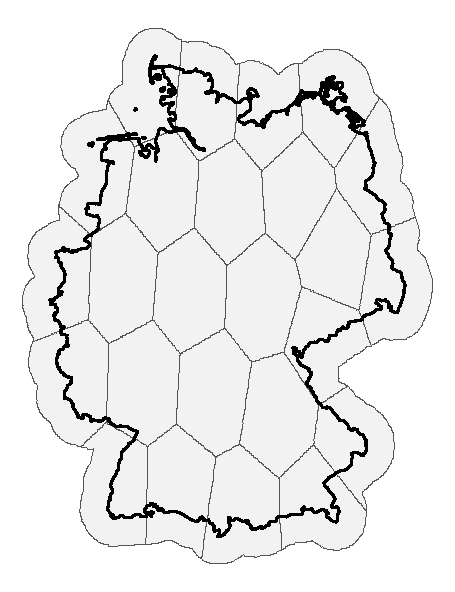
\includegraphics[width=\linewidth]{figures/spatial_weather_load_clusters.pdf}
    \caption{Load}
  \end{subfigure}
  \hfill
  \begin{subfigure}{0.33\textwidth}
    \centering
    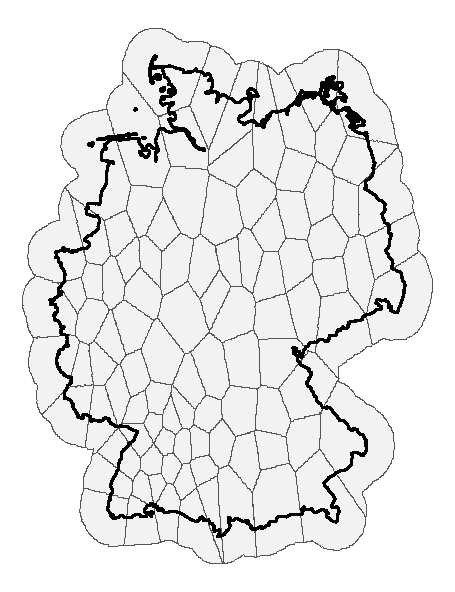
\includegraphics[width=\linewidth]{figures/spatial_weather_solar_clusters.pdf}
    \caption{Solar generation}
  \end{subfigure}
  \hfill
  \begin{subfigure}{0.32\textwidth}
    \centering
    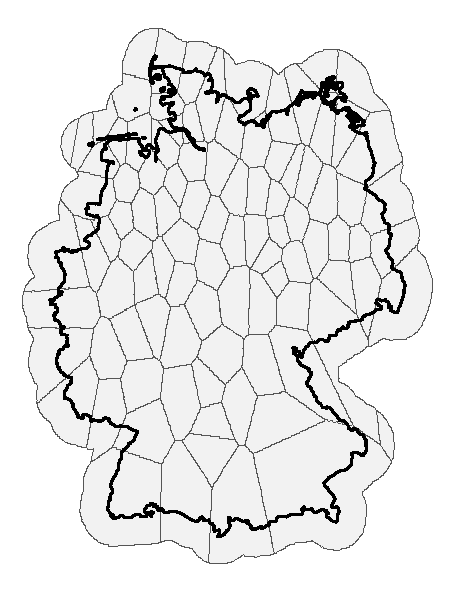
\includegraphics[width=\linewidth]{figures/spatial_weather_wind_clusters.pdf}
    \caption{Wind generation}
  \end{subfigure}
  \caption[Spatial weather representations of the forecasting models.]
  {Spatial weather representations of the forecasting models. Panel~(a) shows
  the 25-cluster weather grid used to construct population-weighted
  load-weather features. Panel~(b) shows the solar representation with 25
  clusters per TSO proxy area. Panel~(c) shows the 100-cluster wind
  representation including offshore sites.}
  \label{fig:spatial_weather_representations}
\end{figure}

\FloatBarrier

\subsubsection{OBTF Load Model}
\label{sec:load_model}

The OBTF load model predicts realized \mbox{DE-LU} load \(L_{d,q}\) for delivery day \(d\)
and MTU \(q\), producing a complete 96-MTU load curve for the
delivery day. The resulting OBTF load forecast is denoted \(\hat{L}_{d,q|d-1}\). The
model is re-estimated in a rolling scheme with a boosted-tree regressor and
uses calendar and holiday variables, lagged realized load, actual load
observed during the morning before forecast creation, weather features, and,
when available, the public \mbox{ENTSO-E} load forecast. For training, realized
load of day \(d-1\) is used only up to the last quarter-hour published before
forecast creation.

The weather block starts from cluster-level forecasts of temperature, dew
point, surface pressure, precipitation, snow depth, cloud cover, solar
radiation, and wind speed. From temperature and dew point, the pipeline derives
relative humidity, vapor-pressure deficit, and heating and cooling degree
variables. Rather than using the 25 cluster series individually, the OBTF load model summarizes
them into a compact set of \mbox{DE-LU}-wide features.
Population-weighted means describe the average weather exposure of consumers,
while daily summaries capture the mean, minimum, maximum, and range of selected
weather variables over the delivery day. Spatial weather quantiles describe the
distribution across clusters at a given MTU, for example the lower, median, and
upper part of the temperature or cloud-cover distribution. They are
descriptive spatial quantiles, not probabilistic forecast quantiles, and are
complemented by cross-cluster spread measures such as ranges and standard
deviations. These features describe whether a weather extreme is confined to one part of the
zone or spread across all of it, which affects aggregate demand beyond what the
population-weighted mean captures.

The model has two operational modes. Before the public load forecast becomes
available, it predicts load directly from the admissible input data. Once the
public load forecast is available, the final model uses a forecast-correction
specification. Let \(L^{\mathrm{ENTSOE}}_{d,q|d-1}\) denote the public
\mbox{ENTSO-E} load forecast, with the correction target defined as the
forecast deviation
\[
  \Delta^{L}_{d,q}
  =
  L_{d,q} - L^{\mathrm{ENTSOE}}_{d,q|d-1},
\]
and adds the predicted correction back to the public forecast,
\[
  \hat{L}_{d,q|d-1}
  =
  L^{\mathrm{ENTSOE}}_{d,q|d-1} + \hat{\Delta}^{L}_{d,q|d-1}.
\]
This treats the \mbox{ENTSO-E} forecast as an admissible baseline and uses the
model to correct remaining errors with the available load, calendar, and
weather information. The public forecast is produced by the system operators
with undisclosed models and inputs \cite{euRegulation543_2013,entsoeTransparency},
which cannot be reconstructed from the open data available here. Correcting it
lets the model add whatever information the public forecast does not already
reflect, namely its systematic errors, information that arrived after it was
issued, such as newer weather runs and the morning's realized load, and
information that was available but is not exploited by the undisclosed model. Predicting this correction rather than the
load level is also favorable in bias-variance terms: the correction is a small
and comparatively stationary target with far less variance than the full load
curve, so a model trained on only a few hundred rolling days estimates it more
reliably than it could estimate load from scratch. The direct mode is relevant for early forecast
creation times in RQ3, while the correction mode is used whenever the public
load forecast is available.

\subsubsection{OBTF Solar Model}
\label{sec:solar_model}

The OBTF solar model predicts realized solar generation \(S_{d,q}\) for all 96
MTUs of the delivery day. The resulting OBTF solar forecast is denoted
\(\hat{S}_{d,q|d-1}\). In the empirical analysis, the model is implemented
with histogram-based boosted trees and estimated on a rolling training window.
It is trained separately for the four German control areas of 50Hertz,
Amprion, TenneT, and TransnetBW, because realized solar generation is published
per control area and the bidding-zone value is essentially their sum. In the
test period, the four areas account for 99.4\% of realized \mbox{DE-LU} solar
generation, with the remainder from Luxembourg. Summing the four area forecasts
to the aggregate OBTF solar forecast therefore mirrors how the realized
value is composed.

The inputs are calendar variables, installed photovoltaic capacity, the position
of the sun, and weather. Realized generation is not used as a lagged input. It
enters only as the training target and through the bias correction described
below. The weather is aggregated over 25 clusters per TSO proxy area
(Section~\ref{sec:weather_representations}) and weighted by installed
photovoltaic capacity. It includes irradiance, temperature,
precipitation, snow, and cloud cover, together with spread measures that
distinguish uniformly cloudy areas from areas where conditions differ across
locations.

The model also uses a physics-based solar baseline, the expected photovoltaic
generation computed from the forecast irradiance and temperature, the position
of the sun, and the installed capacity \cite{antonanzas2016pvForecasting}. The
boosted-tree model then predicts only the deviation from this baseline, which
keeps the forecast physically plausible. Training days on which realized
generation falls far below the baseline under clear-sky conditions, a pattern
more consistent with data errors or curtailment than with weather, are
excluded. Predictions are finally adjusted with a rolling bias correction that
subtracts the average error of recent days, applied per control area and to the
\mbox{DE-LU} total, which also covers the small Luxembourg share.

\subsubsection{OBTF Wind Model}
\label{sec:wind_model}

The OBTF wind model predicts realized wind generation \(W_{d,q}\), including both
onshore and offshore generation, for all 96 MTUs of the delivery day. The
resulting OBTF wind forecast is denoted \(\hat{W}_{d,q|d-1}\). In the
empirical analysis, the model is implemented with histogram-based boosted
trees and estimated on a rolling training window. Onshore and offshore
generation are forecast separately, because they differ in their weather drivers
and spatial concentration and are published as separate production types
\cite{entsoeTransparency}. The two forecasts are then summed to the aggregate
OBTF wind forecast used by the price model.

The inputs are calendar variables, installed wind capacity, and weather. As for
solar, realized generation enters only as the training target and through the
bias correction. The weather is aggregated over 100 clusters including offshore
sites (Section~\ref{sec:weather_representations}), grouped into an offshore
region and five onshore regions, and weighted by installed wind capacity. It
includes wind speed and direction, temperature, and precipitation. Because wind
generation rises nonlinearly with wind speed, the model also uses transformed
wind speeds that approximate a turbine power curve \cite{bandi2016powerCurve}.
From the same \mbox{ICON-D2} run, accessed through Open-Meteo
\cite{openMeteoForecastApi}, it additionally uses wind speeds at typical turbine
hub heights between 80 and 180~m, because generation is especially sensitive to
the wind at hub height \cite{bandi2016powerCurve,foley2012windForecasting}. Predictions are corrected with the same rolling bias
correction as for solar.

\subsubsection{Price Model}
\label{sec:price_model}
\label{sec:price_features}

The price model predicts \(P_{d,q}\) with boosted trees. Before fitting, the
price target is robustly standardized and passed through an inverse hyperbolic
sine transform \cite{uniejewski2018variance}, which stabilizes the variance of
the volatile, spike-prone, and occasionally negative price series, and
predictions are transformed back to price levels for evaluation. As is common in
day-ahead price forecasting, a separate model is fitted for each MTU, because the price level and its drivers differ strongly across the day
\cite{lago2021forecasting}. In RQ2, the base
price forecast \(\hat{P}^{\mathrm{base}}_{d,q|d-1}\) is compared with the
price forecast with OBTF load and renewable-generation forecasts
\(\hat{P}^{\mathrm{gen}}_{d,q|d-1}\). The base price forecast uses price lags,
calendar variables, weather variables, and the published \mbox{ENTSO-E}
day-ahead load forecast, and excludes early cross-market
price signals. The price forecast with OBTF load and renewable-generation forecasts uses the same
variables but replaces the \mbox{ENTSO-E} load forecast with the OBTF
load forecast \(\hat{L}_{d,q|d-1}\) and adds the OBTF combined
renewable-generation forecast \(\hat{G}^{\mathrm{ren}}_{d,q|d-1}\) and the
OBTF residual-load forecast \(\widehat{RL}_{d,q|d-1}\). Because these inputs are themselves model forecasts
rather than realized values, they enter the price model as forecasted inputs
and carry their own forecast error \cite{pagan1984generated}.
Solar and wind enter the price model as a single combined forecast rather than as
two separate inputs, because price formation responds to the total renewable
feed-in that lowers residual load rather than to the split between the two
sources, and a single input keeps the data-limited price model parsimonious. Both
are still forecast separately by their own models.
Residual load denotes load net of renewable generation and is also referred to
as residual demand or net load in the literature
\cite{do2021residualDemand}. It is included as an explicit input in addition
to load and combined renewable generation because it directly represents the
demand that must be met by dispatchable plants, which is the quantity that
sets the marginal price in the merit order \cite{sensfuss2008meritOrder}.
Providing residual load explicitly allows a single tree split to represent
this supply-demand balance, which the boosted-tree model would otherwise have
to recover from load and renewable generation through feature interactions.
This comparison isolates the value of \(\hat{L}_{d,q|d-1}\),
\(\hat{G}^{\mathrm{ren}}_{d,q|d-1}\), and
\(\widehat{RL}_{d,q|d-1}\) because the remaining price lags, calendar
variables, and weather variables are kept the same.
A weather-free price forecast with OBTF load and renewable-generation forecasts,
\(\hat{P}^{\mathrm{gen},-\mathrm{wea}}_{d,q|d-1}\), keeps these forecasts but omits the raw weather features. Because OBTF forecasts are themselves derived from weather, this variant tests
whether they provide a representation of the weather-driven system state that
can substitute for the raw weather inputs.
The cluster-level weather representations are not passed on to the price
model, but are used only inside the OBTF models. These models
first generate final forecasts for load, solar, and wind generation
for each MTU, and the price model receives only the three \mbox{DE-LU} totals
\(\hat{L}_{d,q|d-1}\), \(\hat{G}^{\mathrm{ren}}_{d,q|d-1}\), and
\(\widehat{RL}_{d,q|d-1}\). Intermediate outputs of the OBTF models, such as the separate OBTF solar and wind forecasts before they are combined or any
regional and cluster-level series, are not passed on.
The RQ3 timing experiment then changes the admissible input set according to
the forecast creation time. Additional inputs enter only after their
publication. In particular, reserve-market covariates are included only after
the corresponding Regelleistung.net auction-result blocks are available, and
EXAA prices enter only at the 12:00 cutoff.

Two design choices of the price model are fixed on the development period before
the test period is used. The raw weather variables used by the price model are aggregated to
two spatial clusters, as described in Section~\ref{sec:weather_representations},
and the rolling training window is set to 70 days, the shortest length beyond
which development-period accuracy no longer improves. The window is short
because price relationships shift quickly with fuel prices, renewable capacity,
and season, so recent days are more informative than older ones. These choices
are made with
the same boosted-tree setup for \(\hat{P}^{\mathrm{base}}_{d,q|d-1}\) and
\(\hat{P}^{\mathrm{gen}}_{d,q|d-1}\), so that the RQ2 comparison is not confounded
by a weaker base price forecast.
Appendix~\ref{app:price_results} reports both selection sweeps, including the
steep growth of the daily training cost with the number of weather clusters.

Two simple benchmark forecasts for the price forecast are included in
RQ2. The previous-day naive benchmark uses the realized price curve of delivery
day \(d-1\) as the forecast for day \(d\). The previous-week naive benchmark
uses the realized price curve of delivery day \(d-7\). Both benchmarks are
admissible before the 12:00 gate closure and provide an easily
interpretable baseline for the model-based price forecasts.
Table~\ref{tab:price_model_variants} summarizes the price forecast variants used
in RQ2 and RQ3.

\begin{table}[H]
  \centering
  \small
  \caption[Price forecast model variants and their inputs.]
  {Price forecast variants used in RQ2 and RQ3.}
  \label{tab:price_model_variants}
  \begin{tabular}{@{}>{\raggedright\arraybackslash}p{0.20\textwidth}
                  >{\raggedright\arraybackslash}p{0.70\textwidth}@{}}
    \toprule
    Variant & Description \\
    \midrule
    \(\mathrm{N}_{d-1}\)
    & Previous-day naive price forecast using the realized price curve of
      delivery day \(d-1\). \\
    \addlinespace
    \(\mathrm{N}_{d-7}\)
    & Previous-week naive price forecast using the realized price curve of
      delivery day \(d-7\). \\
    \addlinespace
    \(\hat{P}^{\mathrm{base}}_{d,q|d-1}\)
    & Base price forecast from the boosted-tree model using the
      \mbox{ENTSO-E} load forecast but without OBTF load,
      renewable-generation, and residual-load forecasts. \\
    \addlinespace
    \(\hat{P}^{\mathrm{gen}}_{d,q|d-1}\)
    & Price forecast with OBTF load and renewable-generation forecasts, using the same boosted-tree model
      structure as
      \(\hat{P}^{\mathrm{base}}_{d,q|d-1}\), replacing the \mbox{ENTSO-E} load
      forecast with \(\hat{L}_{d,q|d-1}\) and adding
      \(\hat{G}^{\mathrm{ren}}_{d,q|d-1}\) and
      \(\widehat{RL}_{d,q|d-1}\) as inputs. \\
    \addlinespace
    \(\hat{P}^{\mathrm{gen},-\mathrm{wea}}_{d,q|d-1}\)
    & Weather-free price forecast with OBTF load and renewable-generation
      forecasts. It keeps these forecasts but omits the raw weather features. \\
    \addlinespace
    \(\hat{P}^{t}_{d,q|d-1}\)
    & Cutoff-specific RQ3 price forecast for
      \(t \in \mathcal{T}^{\mathrm{cut}}\), using the weather, morning actuals, OBTF load and renewable-generation forecasts, reserve-market features, public
      \mbox{ENTSO-E} load forecast, and EXAA price signal that are admissible
      at cutoff \(t\). \\
    \bottomrule
  \end{tabular}
\end{table}

\subsection{Experimental Design}
\label{sec:experimental_design}

All experiments share the same temporal setup. Models are re-estimated daily
in a rolling scheme: for each delivery day, each model is trained on a preceding
rolling window of fixed length and then produces the forecast for that day. A
fixed-length rolling window, rather than an expanding one, is used because the
\mbox{DE-LU} system is non-stationary: installed capacity, demand, and price behavior
drift over time, so recent history is more representative of the delivery day,
and bounding the window keeps the model adaptive and the daily training cost
fixed. For the base price model, the development-period sweep shows no
meaningful accuracy gain from an expanding window
(Appendix~\ref{app:price_base_selection}). The
post-transition sample is split into a development period from
1~October~2025 to 31~January~2026 and an out-of-sample test period from
1~February~2026 to 31~July~2026. The development period is used to fix all
design choices, including feature sets, model hyperparameters, and the
rolling-window length, while the test period is held out and used only for the
reported results, so that no design decision depends on test-period
information. The window length is selected per model on the development period,
which for the price model yields 70 days. It is kept short enough that the
price model is trained entirely on post-transition quarter-hourly prices for
every test day, so no reported result relies on pre-transition prices, which are
available only at hourly resolution. Such hourly prices enter only the training
windows of the earliest development days, which reach before 1~October~2025. Evaluations that involve the OBTF wind forecast exclude 7~February~2026, for which no \mbox{ICON-D2} run with wind
fields is archived. The test period spans late winter, spring, and summer, which
matters because load, solar, and wind generation follow different
seasonal patterns and a single-season window would test them unevenly.

\subsubsection{Research Design Matrix}
\label{sec:rq_experiment_mapping}

Table~\ref{tab:rq_experiment_mapping} links the empirical design to the
three RQs. The design covers the accuracy of OBTF forecasts,
their effect on the price forecast, and changes in price forecast performance
as richer information sets become available before gate closure.
The weather representation and spatial aggregation of the OBTF load, solar, and wind models are fixed parts of the implemented pipeline rather than separate
experimental factors. The weather aggregation used by the price model is the one exception,
and it is selected on the development period to keep the base price forecast
in RQ2 a fair control (Section~\ref{sec:weather_representations}).

\begin{table}[H]
  \centering
  \small
  \caption[Mapping of RQs and hypotheses to empirical designs.]
  {Research and hypothesis design matrix.}
  \label{tab:rq_experiment_mapping}
  \begin{tabular}{@{}>{\raggedright\arraybackslash}p{0.13\textwidth}
                  >{\raggedright\arraybackslash}p{0.53\textwidth}
                  >{\raggedright\arraybackslash}p{0.24\textwidth}@{}}
    \toprule
    RQ/H & Empirical design & Outcome assessed \\
    \midrule
    \hyperlink{rq:component_forecast_quality}{RQ1}/\hyperlink{hyp:component_forecast_quality}{H1}
    & \(\hat{L}_{d,q|d-1}\), \(\hat{S}_{d,q|d-1}\), and
      \(\hat{W}_{d,q|d-1}\) are compared with
      \(L^{\mathrm{ENTSOE}}_{d,q|d-1}\),
      \(S^{\mathrm{ENTSOE}}_{d,q|d-1}\), and
      \(W^{\mathrm{ENTSOE}}_{d,q|d-1}\). The realized targets are
      \(L_{d,q}\), \(S_{d,q}\), and \(W_{d,q}\).
    & Forecast quality of the OBTF forecasts \(\hat{L}\), \(\hat{S}\), and
      \(\hat{W}\) relative to \mbox{ENTSO-E} benchmarks \\
    \addlinespace
    \hyperlink{rq:price_impact_generated_forecasts}{RQ2}/\hyperlink{hyp:price_impact_generated_forecasts}{H2}
    & \(\hat{P}^{\mathrm{gen}}_{d,q|d-1}\) is compared with
      \(\hat{P}^{\mathrm{base}}_{d,q|d-1}\). The two forecasts differ only in
      whether \(\hat{L}_{d,q|d-1}\), \(\hat{G}^{\mathrm{ren}}_{d,q|d-1}\), and
      \(\widehat{RL}_{d,q|d-1}\) enter the price model.
    & Effect of the OBTF load and renewable-generation forecasts on price
      forecast accuracy \\
    \addlinespace
    \hyperlink{rq:cutoff_sensitivity}{RQ3}/\hyperlink{hyp:cutoff_sensitivity}{H3}
    & The forecasting pipeline is rerun for
      \(t \in \mathcal{T}^{\mathrm{cut}}\). Inputs are restricted to what is
      available at each cutoff, including the staggered arrival of
      reserve-market results and the late EXAA price signal.
    & Price forecast performance with richer information sets over time \\
    \bottomrule
  \end{tabular}
\end{table}

\FloatBarrier

\subsubsection{RQ1: OBTF Forecasts versus \mbox{ENTSO-E} Forecasts}
\label{sec:rq1_component_forecast_benchmarking}

\hyperlink{rq:component_forecast_quality}{RQ1} is addressed by comparing
\(\hat{L}_{d,q|d-1}\), \(\hat{S}_{d,q|d-1}\), and
\(\hat{W}_{d,q|d-1}\) with the corresponding \mbox{ENTSO-E} day-ahead
forecasts. All forecasts are aligned to the same 96-MTU delivery-day grid and
evaluated against realized load, solar, and wind generation after
delivery. The comparison is deliberately not a same-information comparison:
OBTF forecasts are restricted to the operational information cutoff
of the price pipeline, while the \mbox{ENTSO-E} day-ahead solar and wind
generation benchmark forecasts are not publicly observable before the
12:00 gate closure. This difference reflects the operational setting rather than a flaw of the
design, because the OBTF forecasts have to be created before gate
closure so that they can enter the price model, a constraint the \mbox{ENTSO-E}
solar and wind benchmarks do not face.
Figure~\ref{fig:rq1_component_forecast_design} illustrates this comparison.

\begin{figure}[htbp]
\centering
\begin{tikzpicture}[font=\footnotesize]

% ---- forecasts under comparison ----
\node[fgout=3.2cm] (own) at (-3.2, 0)
  {\textbf{OBTF forecasts}\\\(\hat{L}\), \(\hat{S}\), \(\hat{W}\)};
\node[fgdata=4.5cm, aspect=0.07] (ent) at (3.2, 0)
  {\textbf{\mbox{ENTSO-E} forecasts}\\\mbox{\(L^{\mathrm{ENTSOE}}\), \(S^{\mathrm{ENTSOE}}\), \(W^{\mathrm{ENTSOE}}\)}};

% ---- evaluation row ----
\node[fgeval=3.6cm] (eval) at (0,-2.6)
  {\textbf{Evaluation}\\RMSE, MAE, one-sided\\Giacomini--White test};
\node[fgdata=2.2cm] (real) at (4.4,-2.6)
  {\textbf{Realized values}\\\(L\), \(S\), \(W\)};

\node[fgrq=6.4cm] (rq) at (0,-4.5)
  {\textbf{RQ1:} How do the OBTF forecasts compare with the
   \mbox{ENTSO-E} forecasts?};

% ---- flows ----
\draw[fgflow] (own.south) -- ++(0,-0.55) -| ([xshift=-0.9cm]eval.north);
\draw[fgflow] (ent.south) -- ++(0,-0.55) -| ([xshift=0.9cm]eval.north);
\draw[fgflow] (real.west) -- (eval.east);
\draw[fgflow] (eval.south) -- (rq.north);

\end{tikzpicture}
\caption[OBTF forecast comparison for RQ1.]
{Design of RQ1. The OBTF load, solar, and wind
forecasts and the \mbox{ENTSO-E} forecasts are each scored against the realized
values on a matched panel. The OBTF forecasts use only information
available before the 12:00 deadline. Notation as in
Figure~\ref{fig:system_overview}.}
\label{fig:rq1_component_forecast_design}
\end{figure}


\FloatBarrier

\subsubsection{RQ2: Explicit Load and Renewable-Generation Forecasts in Price Forecasting}
\label{sec:rq2_price_experiments}

\hyperlink{rq:price_impact_generated_forecasts}{RQ2} is addressed by testing
how an explicit representation of load and renewable-generation forecasts
affects the price forecast. This is implemented by adding
\(\hat{L}_{d,q|d-1}\),
\(\hat{G}^{\mathrm{ren}}_{d,q|d-1}\), and
\(\widehat{RL}_{d,q|d-1}\) to the price model. The main
comparison is between \(\hat{P}^{\mathrm{base}}_{d,q|d-1}\) and
\(\hat{P}^{\mathrm{gen}}_{d,q|d-1}\). Both forecasts are produced with the same
boosted-tree model class, the same forecast creation time, the same evaluation
window, and the same price-lag, calendar, and raw weather inputs.
They differ only in whether \(\hat{L}_{d,q|d-1}\),
\(\hat{G}^{\mathrm{ren}}_{d,q|d-1}\), and
\(\widehat{RL}_{d,q|d-1}\) are included.
Since OBTF forecasts are produced by the separate OBTF load, solar, and wind models with task-specific weather representations, this comparison measures
the effect of the explicit load and renewable-generation forecast
representation rather than the effect of an identical raw weather information
set.

A secondary comparison uses the weather-free variant
\(\hat{P}^{\mathrm{gen},-\mathrm{wea}}_{d,q|d-1}\), which keeps OBTF forecasts but omits the raw weather features. Because OBTF forecasts
are derived from weather, comparing
\(\hat{P}^{\mathrm{gen},-\mathrm{wea}}_{d,q|d-1}\) with
\(\hat{P}^{\mathrm{base}}_{d,q|d-1}\) tests whether they can stand in for the raw
weather features, while comparing it with
\(\hat{P}^{\mathrm{gen}}_{d,q|d-1}\) shows whether the raw weather features
still add information beyond OBTF forecasts.

The previous-day and previous-week naive price forecasts are included in this
price forecast comparison. They are not used as benchmarks for the load, solar,
and wind forecasts because RQ1 concerns the quality of
OBTF forecasts relative to the corresponding \mbox{ENTSO-E}
day-ahead forecasts. In RQ2, their role is to show whether the price
models add value beyond simple price persistence.
Figure~\ref{fig:rq3_price_experiments_design} illustrates the RQ2 comparison
together with the weather-free variant and the naive benchmarks.

\begin{figure}[htbp]
\centering
\begin{tikzpicture}[font=\footnotesize]

% ---- price forecast variants ----
\node[fgout=3.5cm] (base) at (-4.9, 0)
  {\textbf{Base forecast}\\\(\hat{P}^{\mathrm{base}}\)\\with the \mbox{ENTSO-E} load forecast};
\node[fgout=3.5cm] (gen) at (0, 0)
  {\textbf{Forecast with OBTF inputs}\\\(\hat{P}^{\mathrm{gen}}\)\\with \(\hat{L}\), \(\hat{G}^{\mathrm{ren}}\), \(\widehat{RL}\) instead};
\node[fgout=3.5cm, fgvar] (wea) at (4.9, 0)
  {\textbf{Weather-free forecast}\\\(\hat{P}^{\mathrm{gen},-\mathrm{wea}}\)\\without raw weather};

% ---- evaluation row ----
\node[fgout=2.4cm, fgvar] (naive) at (-4.9,-2.6)
  {\textbf{Naive benchmarks}\\\(\mathrm{N}_{d-1}\), \(\mathrm{N}_{d-7}\)};
\node[fgeval=3.6cm] (eval) at (0,-2.6)
  {\textbf{Evaluation}\\RMSE, MAE, one-sided\\Giacomini--White test};
\node[fgdata=2.2cm] (real) at (4.9,-2.6)
  {\textbf{Realized}\\\textbf{day-ahead prices}};

\node[fgrq=6.4cm] (rq) at (0,-4.5)
  {\textbf{RQ2:} How do explicit load and renewable-generation forecasts
   affect the day-ahead price forecast?};

% ---- flows ----
\draw[fgflow] (base.south) -- ++(0,-0.55) -| ([xshift=-0.9cm]eval.north);
\draw[fgflow] (gen.south) -- (eval.north);
\draw[fgaux]  (wea.south) -- ++(0,-0.55) -| ([xshift=0.9cm]eval.north);
\draw[fgaux]  (naive.east) -- (eval.west);
\draw[fgflow] (real.west) -- (eval.east);
\draw[fgflow] (eval.south) -- (rq.north);

\end{tikzpicture}
\caption[Price forecast comparison for RQ2.]
{Design of RQ2. The base forecast uses price history, calendar
features, weather, and the \mbox{ENTSO-E} load forecast, while
\(\hat{P}^{\mathrm{gen}}\) replaces the latter with the OBTF load,
renewable-generation, and residual-load forecasts. A weather-free variant and two
naive forecasts serve as secondary comparisons. Notation as in
Figure~\ref{fig:system_overview}.}
\label{fig:rq3_price_experiments_design}
\end{figure}


\FloatBarrier

\subsubsection{RQ3: Richer Information Sets over Time}
\label{sec:cutoff_sensitivity}

\hyperlink{rq:cutoff_sensitivity}{RQ3} is addressed through a
timing experiment that evaluates how electricity price forecast
performance changes with richer information sets over time. The
forecasting pipeline is rerun at the cutoff times
\(\mathcal{T}^{\mathrm{cut}}\) from Section~\ref{sec:operational_information_set}.
At each cutoff, the OBTF load, solar, and wind models of RQ1 and RQ2 are rerun
unchanged with only the inputs available before that time on day \(d-1\), so the OBTF forecasts entering the price model are themselves
cutoff-specific. Realized load and generation enter only up to the last
quarter-hour published at the start of the model run, allowing for a
publication delay of up to one hour \cite{euRegulation543_2013}. All cutoffs use the \mbox{ICON-D2} 06~UTC run, which is
complete about 80~minutes after its start and is therefore admissible from the
10:00 cutoff onward in both winter and summer time. Operationally, the earlier
cutoffs would use an earlier run (Table~\ref{tab:cutoff_accrual}). In the backtest this is not
possible, because the later 09~UTC run is complete only after 12:00 in summer
and the earlier 00 and 03~UTC runs were not archived for the first months of
the test period, so the
earlier cutoffs also use the 06~UTC run (Section~\ref{sec:limitations}). Because
all cutoffs share this weather run, moving
later in the morning can improve the forecasts through more recent realized load
and generation values, reserve-market auction results, and additional inputs
with later publication times. For load, this also
changes the admissible model setup: early cutoffs rely on the direct OBTF load model, while cutoffs after publication of the public
\mbox{ENTSO-E} load forecast can use the forecast-correction mode from
Section~\ref{sec:load_model}. Reserve-market results enter in stages as the
corresponding product auctions become observable: FCR
from 09:00, aFRR from 10:00, and mFRR from 11:00. The EXAA day-ahead price, published around 11:15,
becomes admissible only at the 12:00 cutoff and is included
there as a late price signal.
Table~\ref{tab:cutoff_accrual} lists the admissible inputs at each cutoff. Figure~\ref{fig:cutoff_sensitivity_design} illustrates
the timing experiment.

\begin{figure}[htbp]
\centering
\begin{tikzpicture}[font=\footnotesize]

% ---- time axis of forecast creation times ----
\draw[thick, draw=fgLine, -{Latex[length=2.2mm,width=1.7mm]}] (-5.6,0) -- (5.9,0);
\foreach \x/\l in {-5/07:00, -3/08:00, -1/09:00, 1/10:00, 3/11:00, 5/12:00} {
  \draw[thick, draw=fgLine] (\x,0.08) -- (\x,-0.08);
  \node[font=\scriptsize, above] at (\x,0.1) {\l};
  \node[circle, draw=fgLine, thick, fill=white, inner sep=1.6pt] at (\x,0) {};
}
\node[font=\scriptsize, anchor=west] at (-5.6,0.75)
  {forecast creation time \(t\) on the day before delivery};
\node[font=\scriptsize, anchor=south] at (5,0.55) {gate closure};

% ---- rerun of the pipeline ----
\node[fgproc=10.2cm] (run) at (0,-1.45)
  {\textbf{Rerun the full pipeline at each creation time \(t\)}\\using only inputs admissible at \(t\)};
\foreach \x in {-5,-3,-1,1,3,5}
  \draw[fgflow] (\x,-0.12) -- (\x,0 |- run.north);

% ---- forecasts ----
\node[fgout=3.6cm] (fc) at (0,-3.2)
  {\textbf{Price forecasts}\\\(\hat{P}^{\,t}_{d,q|d-1}\)};
\node[fgout=2.3cm, fgvar] (exaa) at (-4.6,-3.2)
  {\textbf{EXAA-only}\\benchmark at 12:00};

% ---- evaluation ----
\node[fgeval=4.6cm] (eval) at (0,-5.0)
  {\textbf{Evaluation}\\RMSE, MAE, Giacomini--White tests
   against 07:00 and against the preceding time};
\node[fgdata=2.2cm] (real) at (4.6,-5.0)
  {\textbf{Realized}\\\textbf{day-ahead prices}};

\node[fgrq=6.4cm] (rq) at (0,-6.9)
  {\textbf{RQ3:} How does price forecast performance change with richer
   information sets over time?};

% ---- flows ----
\draw[fgflow] (run.south) -- (fc.north);
\draw[fgflow] (fc.south) -- (eval.north);
\draw[fgaux]  (exaa.south) |- (eval.west);
\draw[fgflow] (real.west) -- (eval.east);
\draw[fgflow] (eval.south) -- (rq.north);

\end{tikzpicture}
\caption[Information-set timing experiment for RQ3.]
{Design of RQ3. The full pipeline is rerun at six forecast
creation times from 07:00 to the 12:00 gate closure, each time with only the
information admissible at that time, and the resulting price forecasts are
compared with each other and with a compact EXAA-only benchmark. Notation as in
Figure~\ref{fig:system_overview}.}
\label{fig:cutoff_sensitivity_design}
\end{figure}


\FloatBarrier

\begin{table}[H]
  \centering
  \footnotesize
  \setlength{\tabcolsep}{5pt}
  \caption[Admissible inputs at each forecast creation time.]
  {Admissible inputs at each forecast creation time on day \(d-1\). A dash denotes an input that is not yet admissible.
  \textsuperscript{a}Due to data limitations, the backtest uses the 06~UTC run at
  every cutoff (Section~\ref{sec:limitations}).}
  \label{tab:cutoff_accrual}
  \begin{tabular}{@{}llllllc@{}}
    \toprule
    & \multicolumn{2}{l}{Weather run} & Realized & OBTF & Reserve & \\
    \cmidrule(lr){2-3}
    Cutoff & Operation & Backtest\textsuperscript{a} & data to & load model & products & EXAA \\
    \midrule
    07:00 & 03~UTC & 06~UTC & 05:30 & Direct & \(-\) & \(-\) \\
    08:00 & 03~UTC & 06~UTC & 06:30 & Direct & \(-\) & \(-\) \\
    09:00 & 03~UTC & 06~UTC & 07:30 & Direct & FCR & \(-\) \\
    10:00 & 06~UTC & 06~UTC & 08:30 & Direct & FCR, aFRR & \(-\) \\
    11:00 & 06~UTC & 06~UTC & 09:30 & Correction & FCR, aFRR, mFRR & \(-\) \\
    12:00 & 06~UTC & 06~UTC & 10:30 & Correction & FCR, aFRR, mFRR
      & \(\checkmark\) \\
    \bottomrule
  \end{tabular}
\end{table}

\FloatBarrier

\subsection{Evaluation Framework}
\label{sec:evaluation}

\subsubsection{Evaluation Panel and Error Metrics}
\label{sec:error_metrics}

The evaluation framework is shared across all RQs. Each
comparison uses
out-of-sample forecasts generated under the admissible information set for the
corresponding forecast creation time, over the test period from
1~February~2026 to 31~July~2026 defined in
Section~\ref{sec:experimental_design}. Models within the same RQ
are evaluated on the same delivery days and MTUs. If a model is
missing a forecast for a timestamp in the matched panel, the timestamp is
removed for all models in that specific comparison and the number of
observations is reported.

Let \(e^{m}_{d,q} = Y_{d,q} - \hat{Y}^{\,m}_{d,q|d-1}\) denote the forecast
error of model \(m\), and let \(\mathcal{E}\) be the matched evaluation panel.
All point models are estimated by minimizing squared error, so their forecasts
target the conditional mean of the delivery-period outcome. The primary metric
is therefore the root mean squared error (RMSE),
\[
  \operatorname{RMSE}(m)
  =
  \sqrt{\frac{1}{|\mathcal{E}|}
  \sum_{(d,q)\in\mathcal{E}}
  \bigl(e^{m}_{d,q}\bigr)^{2}},
\]
which rewards accurate estimation of that conditional mean and is the scoring
metric of the Energy-Arena submissions \cite{kleinebrahm2026energyarena}. The
mean absolute error (MAE)
\(\operatorname{MAE}(m) = |\mathcal{E}|^{-1} \sum_{(d,q)\in\mathcal{E}}
|e^{m}_{d,q}|\) is reported alongside it for every comparison, because it is a
standard accuracy metric in the electricity price forecasting literature and,
being expressed in the target unit, aids interpretation and comparison with
published work \cite{lago2021forecasting,hyndman2006another}. Price metrics are
reported in EUR/MWh. Load, solar, and wind
metrics are reported in MW.

\subsubsection{Paired Model Comparisons}
\label{sec:paired_model_comparisons}

Model comparisons are reported as relative RMSE changes. For a reference
forecast \(a\) and a challenger \(b\),
\[
  \Delta\operatorname{RMSE}_{a,b}
  =
  \frac{\operatorname{RMSE}(b) - \operatorname{RMSE}(a)}{\operatorname{RMSE}(a)},
\]
so a negative value means that \(b\) has a lower error than \(a\). When
statistical significance is assessed, the thesis uses the Giacomini-White (GW)
conditional predictive ability test \cite{giacomini2006tests} on the
squared-error loss, consistent with the squared-error training objective and the
RMSE metric. Because the 96 quarter-hourly prices of a delivery day are
forecast jointly, the test is applied to the daily mean loss differential
\(\bar{\delta}_{d}\) across the 96 MTUs. The test uses two instruments,
namely a constant and the previous day's differential \(\bar{\delta}_{d-1}\), so
the test statistic is asymptotically \(\chi^{2}\)-distributed with two degrees of
freedom. The test is
used one-sided, in the direction of the forecast with the lower average loss. The test provides supporting evidence, while the
main interpretation is based on the size, direction, and consistency of the
out-of-sample error differences. When several tests address the same question,
the chance that at least one of them appears significant by coincidence grows
with their number. Within each such family, namely each column of the RQ3 cutoff
results and the three pre-EXAA cutoffs of the reserve ablation, the p-values are
therefore additionally checked with the Holm procedure \cite{holm1979simple}. It
orders the \(m\) p-values of a family from smallest to largest, compares the
smallest with \(5\%/m\), the next with \(5\%/(m-1)\), and so on, and stops at
the first one that exceeds its threshold. This keeps the probability of any
false significant result within the family at 5\%.

\subsubsection{Feature Importance}
\label{sec:feature_importance}

As a diagnostic, the boosted-tree price model is analyzed with SHapley Additive exPlanations (SHAP) values
\cite{lundberg2017shap,lundberg2020treeshap}. SHAP values attribute each individual prediction to
its input features and are aggregated by summation within the feature groups
that make up the price model: price lags, calendar and holiday variables,
weather variables, the EXAA price and reserve-market auction results where
admissible, and the OBTF forecasts
\(\hat{L}_{d,q|d-1}\), \(\hat{G}^{\mathrm{ren}}_{d,q|d-1}\), and
\(\widehat{RL}_{d,q|d-1}\). Because SHAP values are signed, they also show the
direction of each feature's effect, that is, whether it raises or lowers the
forecast, which summary plots across all predictions make visible
\cite{lundberg2017shap,lundberg2020treeshap}, as in
Figure~\ref{fig:rq2_shap_beeswarm}. This analysis helps interpret whether the OBTF forecasts are actually
used by the price model.
